\section{Method}\label{sec:method}

Herein we discuss:
\textbf{(1)} What are~\algname (Sec.~\ref{sec:rekep})?
\textbf{(2)} How to formulate manipulation as a constrained optimization problem with~\algabrvname (Sec.~\ref{sec:task-rekep})?
\textbf{(3)} What is our algorithmic instantiation that can efficiently solve the optimization in real-time (Sec.~\ref{sec:algorithm})?
\textbf{(4)} How to automatically obtain~\algabrvname from RGB-D observations and language instructions (Sec.~\ref{sec:vlm})?

\subsection{\algname (\algabrvname)}\label{sec:rekep}

Herein we define a single instance of~\algabrvname.
For clarity, we assume that a set of $K$ keypoints have been specified (discussed later in Sec.~\ref{sec:vlm}).
Concretely, each keypoint $k_i \in \mathbb{R}^3$ refers to a 3D point on the scene surface with Cartesian coordinates, which is dependent on the task semantics and the environment (e.g., grasp point on the handle, spout).

A single instance of~\algabrvname is a function $f: \mathbb{R}^{K \times 3} \rightarrow \mathbb{R}$ that maps an array of keypoints, denoted as $\bm{k}$, to an unbounded cost, where $f(\bm{k}) \leq 0$ indicates the constraint is satisfied. The function $f$ is implemented as a stateless Python function, containing NumPy~\cite{harris2020array} operations on keypoints, which may be nonlinear and nonconvex.
In essence, one instance of~\algabrvname encodes one desired spatial relation between keypoints, which may belong to robot arm(s), object parts, and other agents.

However, a manipulation task typically involves multiple spatial relations and may have multiple temporally dependent stages where each stage entails different spatial relations.
To this end, we decompose a task into $N$ stages and use~\algabrvname to specify two kinds of constraints for each stage $i \in \{1, \ldots, N\}$:
a set of sub-goal constraints $\mathcal{C}_{\text{sub-goal}}^{(i)} = \{f_{\text{sub-goal},1}^{(i)}(\bm{k}), \ldots, f_{\text{sub-goal},n}^{(i)}(\bm{k})\}$ and a set of path constraints $\mathcal{C}_{\text{path}}^{(i)} = \{f_{\text{path},1}^{(i)}(\bm{k}), \ldots, f_{\text{path},m}^{(i)}(\bm{k})\}$,
where $f_{\text{sub-goal}}^{(i)}$ encodes one keypoint relation to be achieved \textit{at the end of stage $i$}, and $f_{\text{path}}^{(i)}$ encodes one keypoint relation to be satisfied for every state \textit{within stage $i$}.
Consider the pouring task in Fig.~\ref{fig:method}, which consists of three stages: grasp, align, and pour. The stage-1 sub-goal constraint pulls the end-effector towards the teapot handle. Then stage-2 sub-goal constraint specifies that the teapot spout needs to be on top of the cup opening. Additionally, stage-2 path constraint ensures the teapot stays upright to avoid spillage when transported. Finally, the stage-3 sub-goal constraint specifies the desired pouring angle.

\begin{figure}[t]
    \centering
    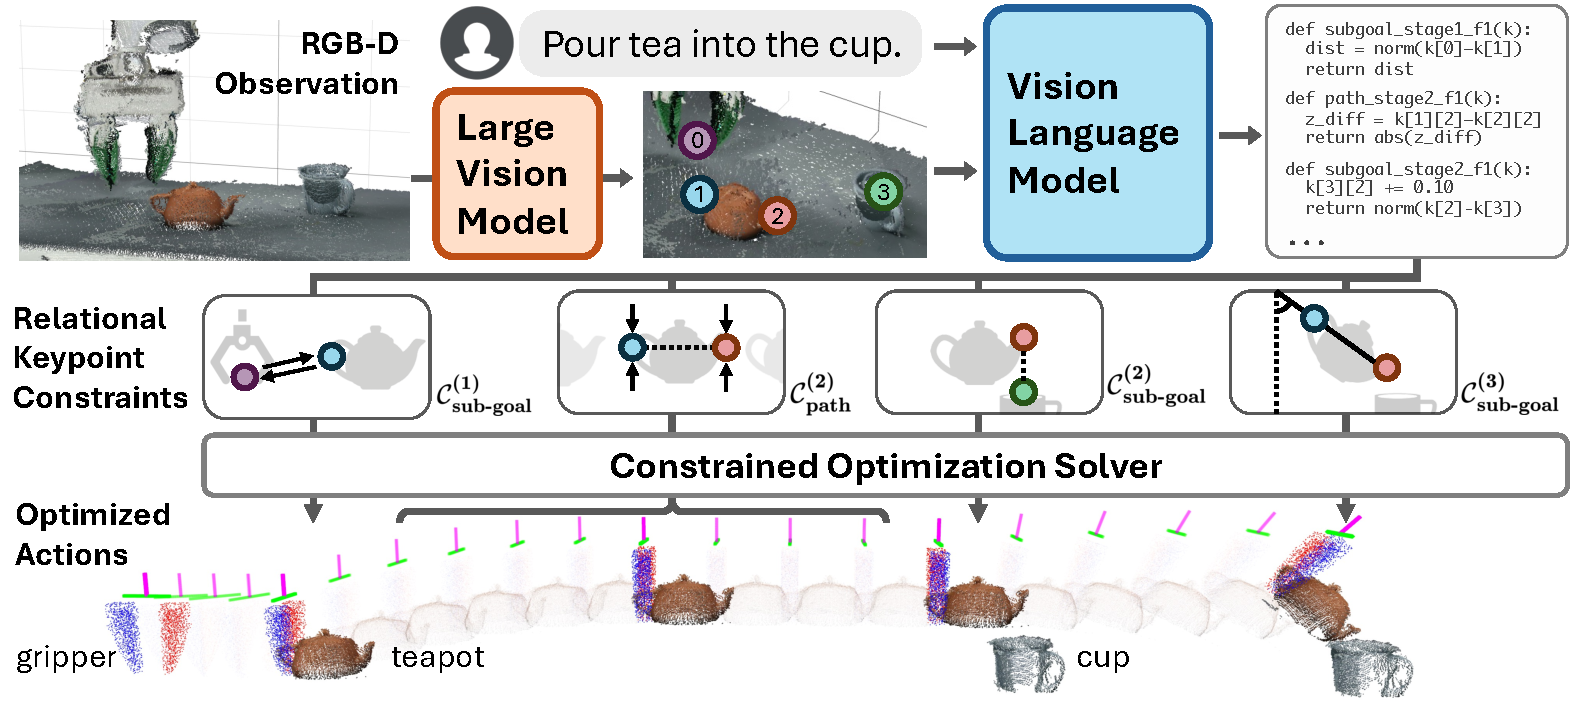
\includegraphics[width=1.0\linewidth]{media/method.pdf}
    \vspace{-1.5em}
    \caption{\small \textbf{Overview of \algabrvname}. DINOv2~\cite{oquab2023dinov2} first proposes keypoints in the scene, which are overlaid on the original RGB image.
    The image and an instruction are fed into GPT-4o~\cite{openai2023gpt} to generate a series of~\algabrvname constraints as python programs that specify desired relations between keypoints at different task stages ($\mathcal{C}_{\text{sub-goal}}^{(i)}$) and any requirement on transitioning behaviors within stages ($\mathcal{C}_{\text{path}}^{i})$. 
    Finally, dense sequence of end-effector actions are obtained by solving the optimization problem subject to generated constraints.}
    \label{fig:method}
    \vspace{-1.35em}
\end{figure}

\subsection{Manipulation Tasks as Constrained Optimization with~\algabrvname}\label{sec:task-rekep}


Using~\algabrvname as a general tool to represent constraints, we adopt the formulation in~\cite{toussaint2022sequence} and show how a manipulation task can be formulated as a constrained optimization problem involving $\mathcal{C}_{\text{sub-goal}}^{(i)}$ and $\mathcal{C}_{\text{path}}^{(i)}$.
We denote the end-effector pose as $\mathbf{e} \in SE(3)$.%
To perform the manipulation task, we aim to obtain the overall discrete-time trajectory $\mathbf{e}_{1:T}$ by formulating the control problem as follows:

\vspace{-2.0em}
\begin{equation}\label{eq:problem}
\begin{split}
\argmin_{\mathbf{e}_{1:T}, g_{1:N}} & \sum_{i=1}^N \left[ \lambda_{\text{sub-goal}}^{(i)}(\mathbf{e}_{g_i}) + \sum_{t=g_{i-1}}^{g_i} \lambda_{\text{path}}^{(i)}(\mathbf{e}_t) \right] \; \text{s.t.}
\end{split}
\quad
\begin{aligned}
& \left\{
\begin{aligned}
& \mathbf{e}_1 = \mathbf{e_{\text{init}}}, \; g_0 = 1, \; 0 < g_i < g_{i+1}\\
& f(\bm{k}_{g_i}) \leq 0, \; \forall f \in \mathcal{C}_{\text{sub-goal}}^{(i)} \\
& f(\bm{k}_t) \leq 0, \; \forall f \in \mathcal{C}_{\text{path}}^{(i)}, \; t = g_{i-1}, \ldots, g_i \\
& \bm{k}_{t+1} = h(\bm{k}_t, \mathbf{e}_t), \; t = 1, \ldots, T-1
\end{aligned}
\right.
\end{aligned}
\end{equation}
\vspace{-2.0em}


where $\mathbf{e}_t$ denotes end-effector pose at time $t$,
$g_i \in \{1, \ldots, T\}$ are the timings of the transition from stage $i$ to $i+1$ which are also auxiliary decision variables,
$\bm{k}_t$ is the array of keypoint positions at time $t$,
$h$ is a forward model of keypoints,
and $\lambda_{\text{sub-goal}}^{(i)}$ and $\lambda_{\text{path}}^{(i)}$ are auxiliary cost functions (e.g., collision avoidance) for the sub-goal and path problems respectively.
Namely, for each stage $i$, the optimization shall find an end-effector pose as next sub-goal, along with its timing, and a sequence of poses $\mathbf{e}_{g_{i-1}:g_{i}}$ that achieves the sub-goal, subject to the given set of~\algabrvname constraints and auxiliary costs.
This formulation can be considered as direct shooting in trajectory optimization~\cite{underactuated}.

\subsection{Decomposition and Algorithmic Instantiation}\label{sec:algorithm}
To solve Eq.~\ref{eq:problem} in real-time,
we employ a decomposition of the full problem and only optimize for the immediate next sub-goal and the corresponding path to reach the sub-goal (pseudo-code in Algorithm~\ref{alg:method}).
All optimization problems are implemented and solved using SciPy~\cite{virtanen2020scipy} with decision variables normalized to $[0, 1]$.
They are initially solved with Dual Annealing~\cite{xiang1997generalized} with SLSQP~\cite{kraft1988software} as local optimizer (around 1 second) and subsequently solved with only local optimizer based on the previous solution at approximately 10 Hz.

\textbf{The Sub-Goal Problem}: We first solve the sub-goal problem to obtain $\mathbf{e}_{g_i}$ for the current stage $i$:
\begin{equation}\label{eq:subgoal}
\begin{aligned}
\argmin_{\mathbf{e}_{g_i}} \; \lambda_{\text{sub-goal}}^{(i)}(\mathbf{e}_{g_i}) \quad
\text{s.t.} \quad
f(\bm{k}_{g_i}) \leq 0, \; \forall f \in \mathcal{C}_{\text{sub-goal}}^{(i)}
\end{aligned}
\end{equation}
where $\lambda_{\text{sub-goal}}$ subsumes auxiliary control costs: scene collision avoidance, reachability, pose regularization, solution consistency, and self-collision for bimanual setup (details in \ref{app:subgoal}).
Namely, Eq.~\ref{eq:subgoal} attempts to find a sub-goal that satisfies $\mathcal{C}_{\text{sub-goal}}^{i}$ while minimizing the auxiliary costs.
If a stage is concerned with grasping, a grasp metric is also included. In this work, we use AnyGrasp~\cite{fang2023anygrasp}\footnote{Since AnyGrasp is a grasp detector instead of a metric and is computationally expensive to run in optimization loops, we always return the grasp closest to a specified ``grasp keypoint'' by exploiting the fact that~\algabrvname related to grasping always associates a dummy keypoint on the end-effector and one actual keypoint.}.

\textbf{The Path Problem}: After obtaining sub-goal $\mathbf{e}_{g_i}$, we solve for a trajectory $\mathbf{e}_{t:g_i}$ starting from current end-effector pose $\mathbf{e}_t$ to the sub-goal $\mathbf{e}_{g_i}$:
\begin{equation}\label{eq:path}
\begin{aligned}
\argmin_{\mathbf{e}_{t:g_i}, g_i} \; \lambda_{\text{path}}^{(i)}(\mathbf{e}_{t:g_i}) \quad
\text{s.t.} \quad
& f(\bm{k}_{\hat{t}}) \leq 0, \quad \forall f \in \mathcal{C}_{\text{path}}^{(i)}, \quad \hat{t} = t, \ldots, g_i
\end{aligned}
\end{equation}
where $\lambda_{\text{path}}$ subsumes the following auxiliary control costs: scene collision avoidance, reachability, path length, solution consistency, and self-collision in the case of bimanual setup (details in \ref{app:path}).
If the distance to the sub-goal $\mathbf{e}_{g_i}$ is within a small tolerance $\epsilon$, we progress to the next stage $i+1$.


\textbf{Backtracking}: Although the sub-problems can be solved at a real-time frequency to react to external disturbances within a stage, it is imperative that the system can replan across stages if any sub-goal constraint from the last stage no longer holds (e.g., cup taken out of the gripper in the pouring task). Specifically, in every control loop, we check for violation of $\mathcal{C}_{\text{path}}^{(i)}$. If one is found, we iteratively backtrack to a previous stage $j$ such that $\mathcal{C}_{\text{path}}^{(j)}$ is satisfied.

\textbf{Forward Models for Keypoints}:
To solve Eq.~\ref{eq:subgoal} and Eq.~\ref{eq:path}, one must utilize a forward model $h$ that estimates $\Delta \bm{k}$ from $\Delta \mathbf{e}$ in the optimization process.
As in prior work~\cite{manuelli2019kpam}, we make the rigidity assumption between the end-effector and the ``grasped keypoints'' (a rigid group of keypoints that belong to the same object or part; obtained from the segmentation model as described in Sec.~\ref{sec:vlm}.).
Namely, given a change in the end-effector pose $\Delta \mathbf{e}$, we can calculate the change in keypoint positions by applying the same relative rigid transformation $\bm{k}'[\text{grasped}] = \mathbf{T}_{\Delta \mathbf{e}} \cdot \bm{k}[\text{grasped}]$, while assuming other keypoints stay static.
We note that this is a ``local'' assumption in that it is only assumed to hold for the short duration (0.1s) that the problem is solved.
Actual keypoint positions are tracked using visual input at 20 Hz and used in every new problem.
For more challenging scenarios (e.g., dynamic or contact-rich tasks), a learned or physics-based model may be used.




\subsection{Keypoint Proposal and \algabrvname Generation}\label{sec:vlm}
To enable the system to perform tasks in-the-wild given a free-form task instruction, we devise a pipeline using large vision models and vision-language models for keypoint proposal and \algabrvname generation, which are respectively discussed as follows:

\textbf{Keypoint Proposal}:
Given an RGB image $\mathbb{R}^{h \times w \times 3}$,
we first extract the patch-wise features $\mathbf{F}_{\text{patch}} \in \mathbb{R}^{h' \times w' \times d}$ from DINOv2~\cite{oquab2023dinov2}.
Then we perform bilinear interpolation to upsample the features to the original image size, $\mathbf{F}_{\text{interp}} \in \mathbb{R}^{h \times w \times d}$.
To ensure the proposal covers all relevant objects in the scene, we extract all masks $\mathbf{M} = \{\mathbf{m}_1, \mathbf{m}_2, \ldots, \mathbf{m}_n\}$ in the scene using Segment Anything (SAM)~\cite{kirillov2023segment}.
For each mask $j$, we cluster the masked features $\mathbf{F}_{\text{interp}}[\mathbf{m}_j]$ using $k$-means with $k=5$ with a cosine-similarity metric.
The centroids of the clusters are used as keypoint candidates, which are projected to a world coordinate $\mathbb{R}^3$ using a calibrated RGB-D camera.
Candidates that are within $8$cm of others are filtered out.
Overall, we find that this procedure is adept at identifying a large percentage of fine-grained and semantically meaningful regions of objects. 

\begin{figure}[t]
    \centering
    \includegraphics[width=1.0\linewidth]{media/task-viz.pdf}
    \caption{\small \textbf{Experiment tasks and visualization of optimization results.} Seven tasks are designed to validate different aspects of our system, including in-the-wild specification with commonsense knowledge, multi-stage tasks with spatio-temporal dependencies, bimanual coordination with geometric awareness, and reactiveness when collaborating with humans and under disturbances.}
    \label{fig:viz}
    \vspace{-1.55em}
\end{figure}

\textbf{\algabrvname Generation}:
After obtaining the keypoint candidates, we overlay them on the original RGB image with numerical marks.
Coupled with the language instruction of the task, we then use visual prompting to query GPT-4o~\cite{openai2023gpt} to generate the number of required stages and the corresponding sub-goal constraints $\mathcal{C}_{\text{sub-goal}}^{(i)}$ and path constraints $\mathcal{C}_{\text{path}}^{(i)}$ for each stage $i$ (prompts are in~\ref{app:prompt}).
Notably, the functions do not directly manipulate the numerical values of the keypoint positions.
Rather, we exploit the strength of VLM to specify spatial relations as \emph{arithmetic operations}, such as L2 distance or dot product between keypoints, that are only instantiated when invoked with actual keypoint positions tracked by a specialized 3D tracker.
Furthermore, an important advantage of using arithmetic operations on a set of keypoint positions is that it can specify 3D rotations in full $SO(3)$ when sufficient points are provided and rigidity between relevant points is enforced, but this is done only when needed depending on task semantic.
This enables VLM to reason about 3D rotations with arithmetic operations \emph{in 3D Cartesian space}, effectively circumventing the need for dealing with alternative 3D rotation representation and the need for performing numerical computation.
